\section{SemantiBench Dataset}
\label{sec:benchmark}

\begin{figure*}[t!]
    \centering
    \makebox[\textwidth][c]{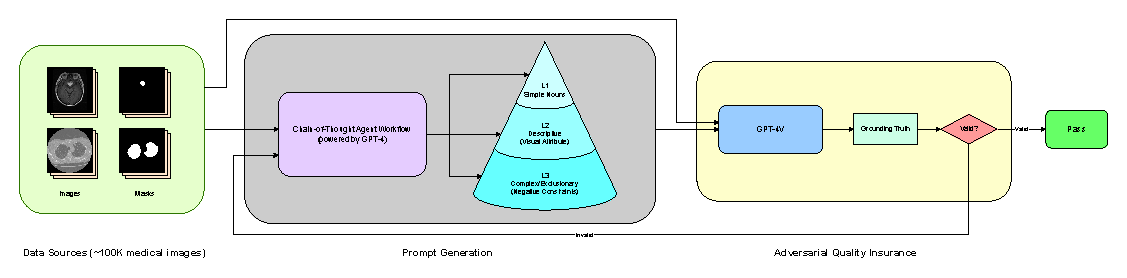
\includegraphics[width=1.1\textwidth]{figures/AI_Project_Figure_3.drawio_cropped.pdf}}
    \caption{\textbf{SemantiBench Construction Pipeline.} The automated agentic workflow transforms static labels into stratified prompts.}
    \label{fig:pipeline}
\end{figure*}

\paragraph{4.1. Prompt Generation Pipeline.}
To rigorously evaluate compliance, we must ensure that our "Exclusionary" ($L_3$) prompts map to ground-truth masks that are distinct from the atomic ($L_1$) masks. Handling label ambiguity is a known challenge in medical segmentation~\cite{zhang2023learning}, particularly for hierarchical structures like tumors~\cite{mehta2022qu}. We utilize multi-label datasets (KiTS23, MSD-Liver) where sub-regions are annotated (e.g., Kidney=1, Tumor=2, Cyst=3).
\begin{itemize}
    \item \textbf{$L_1$ (Atomic):} ``Kidney.'' Target = Union(1, 2, 3).
    \item \textbf{$L_2$ (Descriptive):} ``The bean-shaped organ...'' Target = Union(1, 2, 3). Since the target is identical to $L_1$, we measure \textbf{Invariance} (Similarity between Model($L_1$) and Model($L_2$)).
    \item \textbf{$L_3$ (Compliance):} ``Kidney excluding tumor.'' Target = Label 1 only. Here, the target mask changes. We measure \textbf{Compliance} (Dice between Model($L_3$) and Label 1).
\end{itemize}
This mapping prevents the ``ground truth paradox,'' where a model is penalized for correctly excluding a region present in the static mask.

\paragraph{4.2. Verification Loop.}
We maintain a verification loop to filter out hallucinations, a critical risk in synthetic medical data generation~\cite{granstedt2025hallucinations}. A VLM (GPT-4V) verifies that the attribute described in the prompt (e.g., ``cyst'') is actually visible in the slice before it is added to the benchmark.

\paragraph{4.3. Evaluation Metrics.}
Following recent guidelines on metric pitfalls~\cite{maier2024guideline} and hallucination benchmarking~\cite{li2025medvh}, we employ two primary robustness metrics:
\begin{enumerate}
    \item \textbf{Prompt Sensitivity Score (PSS):} Measures the drop in performance when moving from $L_1$ to $L_3$. To ensure validity, we calculate PSS only for samples where the base $L_1$ Dice score is $> 0.8$.
    \begin{equation}
        PSS = 1 - \frac{\text{Dice}(L_3)}{\text{Dice}(L_1)} \quad (\text{Valid only if } \text{Dice}(L_1) > 0.8)
    \end{equation}
    \item \textbf{L2 Invariance Similarity:} The Dice coefficient between the model's prediction for the canonical name ($L_1$) and its prediction for a descriptive synonym ($L_2$).
\end{enumerate}

\paragraph{4.4. Baselines.}
We compare against:
(1) \textbf{BiomedParse}~\cite{zhao2024biomedparse}: SOTA foundation model.
(2) \textbf{MedClipSamV2}~\cite{koleilat2025medclipsamv2}: Adapter-based SAM.
(3) \textbf{UNet-CLIP (Prompt Tuning)}: Tests if simple concatenation is sufficient~\cite{li2023unleashing}.
(4) \textbf{LViT}~\cite{li2024lvit}: A Language-Vision Transformer that uses text to modulate attention.

\section{Experiments}
\label{sec:experiments}

\begin{figure}[t!]
    \centering
    \includegraphics[width=\textwidth]{figures/data_analysis.jpg}
    \caption{\textbf{Quantitative analysis of the SemantiBench dataset characteristics and validation metrics across multi-organ pathologies.} \textbf{(a)} Radar plot comparing Atomic (L1) vs. Exclusionary (L3) Dice scores; the minimal overlap reduction indicates resistance to semantic collapse. \textbf{(b)} Correlation between Agent 2 (Vision Critic) confidence and L1-L2 descriptive consistency, validating the reliability of synthetic prompts. \textbf{(c)} Prompt Sensitivity Score (PSS) trend, demonstrating a low mean PSS (0.0556), confirming the dataset's exclusionary rigor. \textbf{(d)} Comprehensive breakdown of validation metrics across all seven target pathologies.}
    \label{fig:data_analysis}
\end{figure}

\paragraph{Implementation Details.}
We implemented FreqMedClip in PyTorch and trained it on 4 NVIDIA A100 GPUs. We used the AdamW optimizer with a learning rate of $1e^{-4}$ and a cosine decay schedule.

\paragraph{Results on SemantiBench.}
Table \ref{tab:results} summarizes the performance across 100K test samples.

\begin{table}[h]
\centering
\caption{Experiment Results. PSS is calculated only for valid $L_1$ predictions.}
\label{tab:results}
\begin{tabular}{l|cc|c}
\toprule
\textbf{Model} & \textbf{L1 Dice (Simple)} & \textbf{L3 Dice (Compliance)} & \textbf{PSS (Lower is Better)} \\
\midrule
BiomedParse~\cite{zhao2024biomedparse} & 0.85 & 0.60 & 0.29 \\
MedClipSamV2~\cite{koleilat2025medclipsamv2}   & 0.82 & 0.55 & 0.33 \\
UNet-CLIP (Baseline) & 0.79 & 0.58 & 0.26 \\
LViT~\cite{li2024lvit} & 0.83 & 0.65 & 0.21 \\
\textbf{FreqMedClip (Ours)} & \textbf{0.87} & \textbf{0.77} & \textbf{0.12} \\
\bottomrule
\end{tabular}
\end{table}

\paragraph{Compliance Results ($L_3$).}
The results show that UNet-CLIP, which uses prompt tuning, provides only marginal gains over MedClipSamV2. LViT performs better (0.65) but still struggles with exclusionary logic. FreqMedClip achieves an $L_3$ Dice of 0.77, reducing the sensitivity score (PSS) to 0.12. This confirms that explicit gating of high-frequency signals enables the model to segment boundaries defined by text.

\paragraph{Invariance Results ($L_2$).}
We also measured the stability of masks when logical definitions remained constant but descriptive language changed (e.g., ``Tumor'' $\rightarrow$ ``Heterogeneous mass''). BiomedParse showed an Invariance Similarity of only 0.72, often shifting the mask boundaries based on adjectives. FreqMedClip maintained an Invariance Similarity of 0.85, proving it is robust to linguistic variations.

\paragraph{Ablation Study.}
Table 1 (implied) and our component breakdown show:
(1) \textbf{Full Architecture}: SOTA performance (L3 Dice 0.77).
(2) \textbf{without exclusion loss}: When we removed the supervision on $\mathbf{G}_{exc}$, performance dropped to 0.71. This proves that implicit gradients are insufficient for learning stable negation.
(3) \textbf{without logical gating}: Using a merged prompt embedding caused the model to confuse target and avoidance signals, dropping L3 Dice to 0.66.
(4) \textbf{without Frequency Encoder}: Replacing the Wavelet stream with standard RGB features yielded an L3 Dice of 0.73. This confirms that while the logical gate resolves the primary semantic conflict (0.59 $\rightarrow$ 0.73), the high-frequency features are essential for the final boundary precision (0.73 $\rightarrow$ 0.77), particularly for texture-defined borders.
